\section{MAS Traffic Simulator Backend}\label{sec:backend}
This section describes the backend part of the implemented MAS traffic simulator. First, we give an overview of the MAS architecture.  In \autoref{subsec:agents} we characterize the different types of implemented agents. Finally, this section ends with an outline of the simulation.
\subsection{Backend Architecture}\label{subsec:backendArchitecture}
Several multi-agent traffic/transport simulation frameworks were mentioned in \autoref{sec:relatedWork}, but for this project, we decided to implement our own traffic simulation.  
Building a multi-agent system from the ground up can be a laborious task. Therefore, it seemed to be a good idea to utilize a multi-agent framework.
The most popular one is probably the JAVA Agent DEvelopment Framework (JADE). Nevertheless, we wanted to implement the simulation in the Python programming language.   We tried osBrain and SPADE and chose the latter one because of it's subjectively better usability.

SPADE allows building concurrent multi-agent systems by utilizing the Python asyncio library. For agent communication, it uses the Extensible Messaging and Presence Protocol (XMPP). Thus, it is necessary to run an XMPP server in order to use SPADE. We chose Prosody as recommended by SPADE, but it is possible to use any other XMPP server. Using XMPP might be useful when agents not only need to communicate with other agents but also with humans. 



Furthermore, SPADE supports the FIPA Agent Communication Language (ACL). While we incorporate FIPA ACL parameters like sender, receiver, performative and content in our agents, we only use a couple of performatives like receive and inform. But those are not critical to the functionality of our agents. 
\begin{figure}[h]
	\centering
	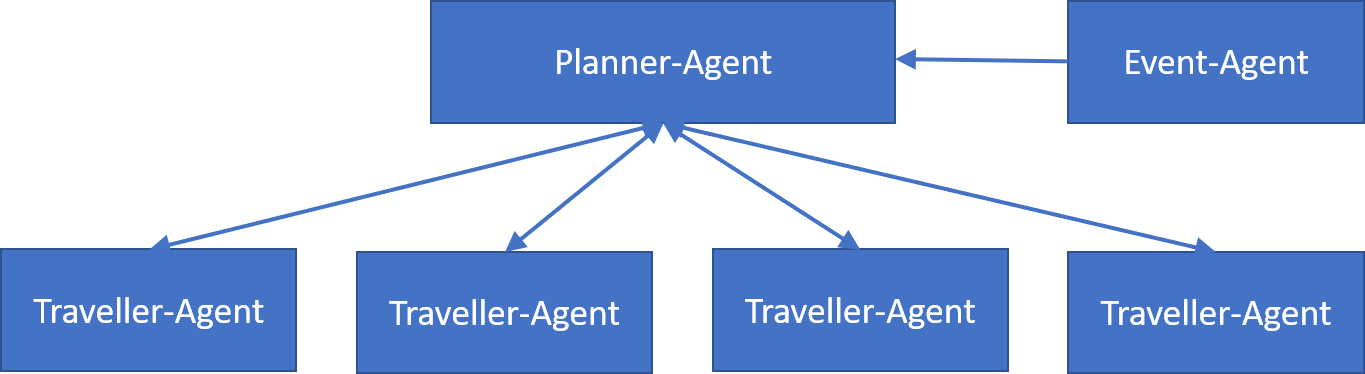
\includegraphics[width=0.8\textwidth]{images/backend_architecture.png}
	\caption{Backend architecture overview}
	\label{fig:backend_architecture}
\end{figure}

To achieve the goals for this project, we decided to use an architecture that focuses on a planner agent. All traveller agents connect to the planner agent in order to receive real-time information while moving on a graph. An event agent is able to trigger events in the simulation.
\autoref{fig:backend_architecture} gives a rough overview of the architecture. The following section will describe the different agent types in detail.


\subsection{Implemented Agents}\label{subsec:agents}

\subsubsection{Planner Agent}\label{subsubsec:planner_agent}
The planner agent is responsible for keeping track of the traveller agents and their positions on the graph. When started, the planner agent loads a graph.  It is assumed that the distances between nodes and the maximum capacities $k_{c}$ of the edges are defined. Next, the free flow speed $\alpha$ and the congestion speed $\beta$ have to be specified. While traveller agents can also be spawned with a specific maximum free flow speed, for simplicity reasons, we decided to use a global approach. This approach can be compared to speed limits on highways.

The planner agent is able to provide travellers with shortest paths and current possible travel times.  In order to fulfill this function, the planner updates the travel times each time an agent enters or exits an edge in the graph.
The travel time for an edge can be computed with $ t = \frac{distance}{s} $ where the speed $ s $ is calculated by \autoref{eq:edge_speed} in dependence of the current edge density $k$ like proposed by \cite{mastio2015towards}. Additionally, we set the minimum speed to 10.

\begin{equation}\label{eq:edge_speed}
s = 
\begin{cases}
\alpha, & \text{if}\ k \leq k_{c} \\
-\beta(k - k_{c}) + \alpha*k_{c}, & \text{otherwise}
\end{cases}
\end{equation}

\autoref{fig:speed_function} shows an example with $\alpha = 100$, $\beta=20$, and $k_{c} = 20$.

\begin{figure}[h]
	\centering
	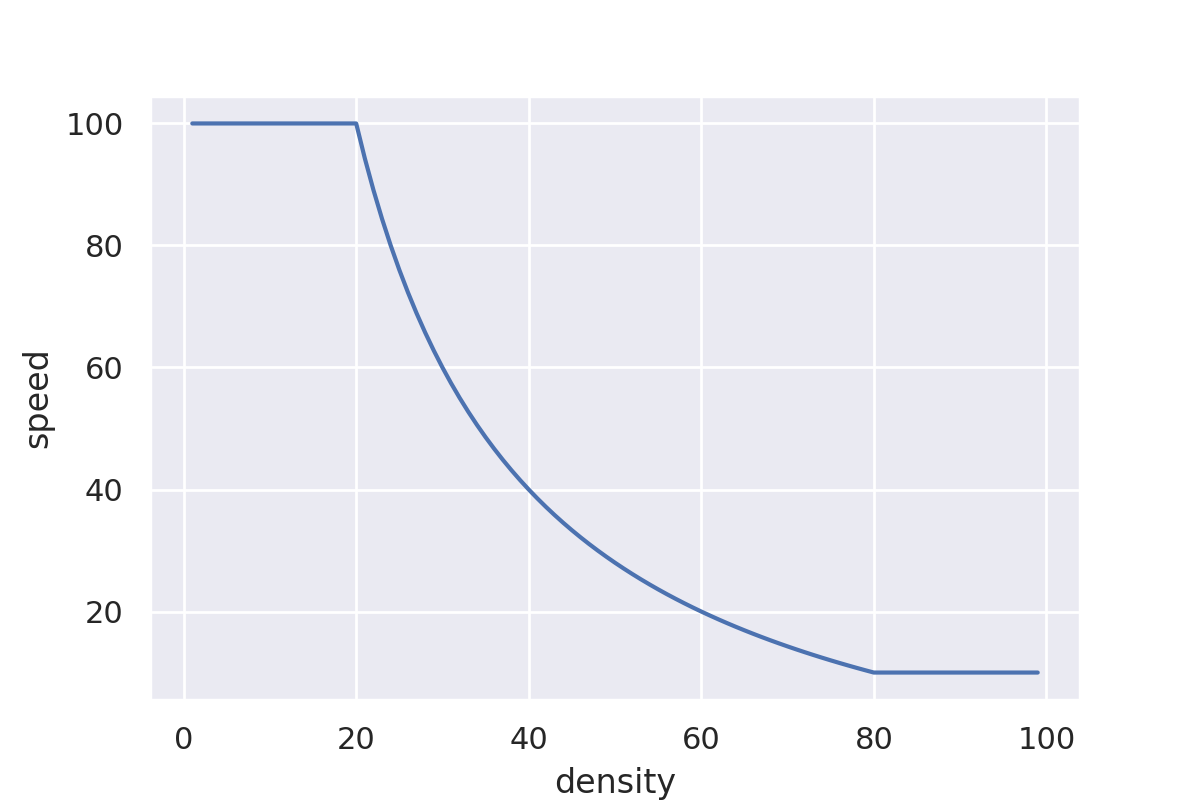
\includegraphics[width=0.5\textwidth]{images/speed.png}
	\caption{Speed in relation to edge density}
	\label{fig:speed_function}
\end{figure}

Besides, the planner agent also logs all interactions with the travellers and the event agent. For example, when a traveller receives a route or a travel time for an edge, the planner saves this information. If the same agent receives an updated route or travel time, the planner registers those changes. Such information can be used to analyze the traffic simulation and also to visualize it as described in \autoref{sec:frontend}.


Technically, the planner agent is utilizing SPADE's cyclic behavior. The cyclic behavior allows an agent to perform an action repeatedly.  In our case, he listens on several endpoints for messages from other agents and processes them.

\subsubsection{Traveller Agents}\label{subsubsec:traveller}
We implemented two different types of traveller agents. Local traveller agents compute their optimal route only at the beginning of their journey. They can only access information from the initial graph like edge distances for example.  
Global agents update their route at each node, incorporating the current traffic situation. 
Traveller agents can be initialized with predefined start and destination nodes. Alternatively, start and destination node can also be selected randomly from the set of nodes in the graph.

Both agent types are built on top of SPADE's finite state machine behavior. When an agent is created, he starts in the \textit{spawn} state. In this state, he will send a message with the current timestamp to the planner agent. The planner agent will use this information for logging reasons. 
If a global agent is in the \textit{get\_route} state, he will send a message to the planner agent with his current node and his destination node. After that, he will wait for an answer from the planner agent containing the next node and the maximum speed. Local agents do not get route updates. They will only receive the maximum speed. 

Next, the traveller agent will send another message to the planner to inform him that he is going to start his journey. The planner will increment the density of the edge and recompute the maximum speed. When in the \textit{drive} state, traveller agents will compute the travel time necessary to traverse the current edge and sleep for this duration.
In the \textit{end\_edge} state, travellers send another message to the planner. The planner will update the maximum speed of the edge accordingly. If the reached node is equal to the destination node, the agent will transition into the \textit{arrived} state. Otherwise, he will go back into the \textit{get\_route} state. In the \textit{arrived} state, the traveller agent will send a last message to the planner for logging reasons. \autoref{fig:fsm} gives a graphical overview of the implemented finite state machine.

\begin{figure}[h]
	\centering
	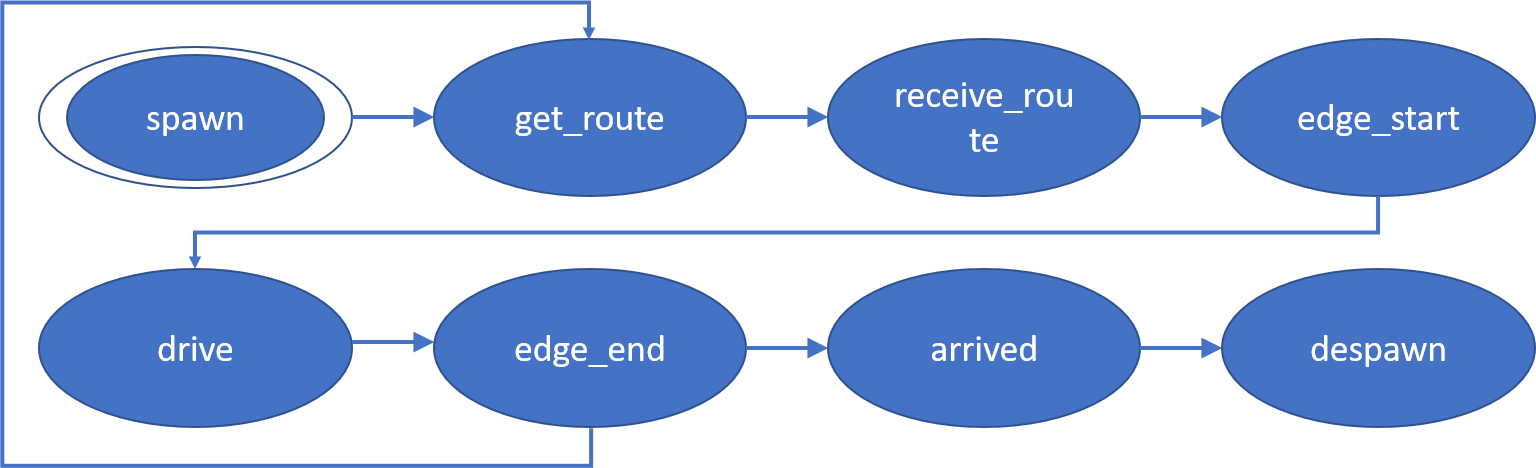
\includegraphics[width=1\textwidth]{images/FSM.png}
	\caption{Finite state machine for the traveller agent}
	\label{fig:fsm}
\end{figure}

\subsubsection{Event Agent}\label{subsubsec:event}
The event agent is able to trigger different events which can have an impact on the simulation in several ways. The \textit{road\_works\_start} event selects an edge in the graph and a factor in the range from 0.2 to 0.9 randomly. This information will be sent to the planner agent. The planner agent will multiply the maximum speed of the edge with the selected factor thus the travel times on this edge will be raised. Such roadworks last until the\textit{ road\_works\_end event} is performed by the event agent. This event resets the factor of an affected edge to 1.

The \textit{spawn\_random\_agents} event spawns a random amount of agents with randomized start and destination nodes. An arbitrary amount of agents with the same start and destination node will be spawned by the \textit{spawn\_agents event}.

The period, at which events occur and also the maximum number of events per simulation can be adjusted in the \textit{file event\_agent.py}.



\subsection{Utilized Graph}\label{subsec:graph}
Traffic networks are not randomly generated. In most cases, they are elaborately planned networks that have to meet the requirements of high traffic volumes. That is why we avoid random graphs and instead use so-called scale-free networks. Specifically, we use the Barabási-Albert  model from the NetworkX package.  In this model, a node is more likely to be connected with a node that already has many edges. Such a node can be compared to a large motorway junction.

The file \textit{graphcreator.py} generates Barabási-Albert graphs \cite{barabasi1999graph} which can be used with our simulation. It will assign a distance to the edges ranging from 1 to 1000. The capacity of the edges will be chosen according to a given distribution. The distribution can be adjusted by changing the global variable \textit{CAPACITIES}.

Finally, to use a created graph in the simulation, the path to the graph has to be set in \textit{simulation.py}. The simulation will create several log files. The following section will describe how they are used by the frontend.
% no timestepping but rather timestamping (event-based)
% Car Agent types be LOCAL, SEMI_LOCAL, GLOBAL
% respective type of information available / being queried from planner-agent

% Public transit is due to complexity of formal representation of timetables not done.

% NOTE: persisted info of sim run (logging info etc.) will be covered in detail in frontend (as this is basically what's being displayed and red from NodeJS app). This `Backend` section needed to describe which parts of the agents save which of their information, but no detail regarding how these are being put together later need be explained here just now. 